\section{The Torque from an Elliptic Ring}
The torque imparted by a force \( \vec{F} \) on a point mass at \( \vec{r} \) is given by
\begin{equation}
    \vec{\tau} = \vec{r} \times \vec{F}
\end{equation}
The gravitational force on a mass \( m \) at \( \vec{r} \) exerted by a gravitational potential \( \Phi \) is given by
\begin{equation}
    \vec{F}(\vec{r}) = -m\vec{\nabla} \Phi(\vec{r})
\end{equation}
so we have that the torque is equal to
\begin{equation}
    \vec{\tau} = -m\vec{r} \times \vec{\nabla} \Phi(\vec{r})
\end{equation}
Lets say we have another elliptic ring centred at the origin and with the same eccentricity,
with radius \( R_2 \) and rotated by an angle \( \alpha \) anti-clockwise. The torque
imparted by the first elliptic ring onto the second elliptic ring can be calculated by
first considering the torque on a line segment of the second elliptic ring
\begin{equation}
    \delta \tau = -\nu \vec{r} \times \vec{\nabla} \Phi(\vec{r}) \delta s
\end{equation}
where \( \nu = \frac{m}{l} \) is the mass per unit length of the second elliptic ring, \( M \) is the
total mass of the second elliptic ring and \( L \) is the perimeter of the second elliptic ring. The total
torque is then just the integral over the entire ring
\begin{equation}
    \tau
    = -\nu \int \vec{r} \times \vec{\nabla} \Phi(\vec{r}) \,{}\,{} \mathrm{d}s
    = -a\nu R \int_{0}^{2\pi} \sqrt{1 - e^2\cos^2{\theta}} \left(\vec{r} \times \vec{\nabla} \Phi(\vec{r})\right) \,\,{} \mathrm{d}\phi
\end{equation}
These integrals do not have closed form solutions and so can only be solved via numerical methods.

\subsection{Particle Approximation}
One method to approximate the torque on the second ring, is to approximate the ring by
dividing it into a \( N \) point particles uniformly distributed around the
ring\footnote{The distance between each point on the ellipse is the same arc length.}.
The torque exerted by the first elliptic ring
only\footnote{There are no forces between particles part of the same elliptic ring, as the rings are rigid}
is calculated for all \( N \) particles, and then total torque is simply the sum of the
torques on the \( N \) particles.
\begin{equation}
    \tau \approx \sum_{n=1}^{N} \tau_n = \frac{M}{N} \sum_{n=1}^{N} \vec{r_n} \times \vec{\nabla} \Phi(\vec{r_n})
\end{equation}
The masses of the particles is \( M_n = \frac{M}{N} \) where \( M \) is the total mass of the second elliptic ring and \( N \) is
number of particles.

\subsection{Results}
Let there be two elliptic rings with equal masses \( 1000 \),
radii \( R_1 = 1 \) and \( R_2 = 3 \) and axes ratio \( \frac{b}{a} = 2 \).
We will rotate the second elliptic ring for a full revolution and calculate the torque along the
\( z \)-axis on the second elliptic ring by exerted by the first elliptic ring and vice versa.

\begin{figure}[h!]
    \begin{center}
        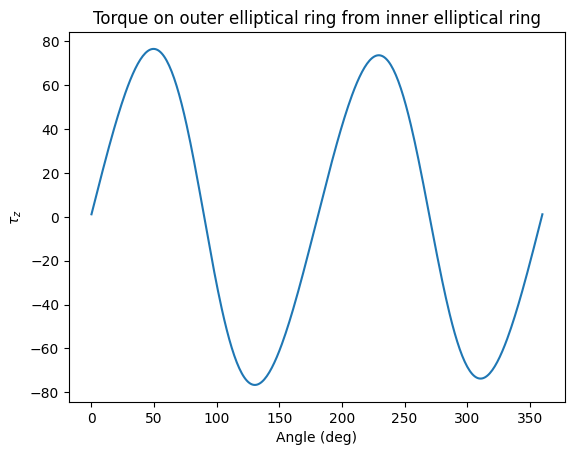
\includegraphics[scale=0.9]{resources/torque_on_outer_ellipse.png}
        \caption{Torque exerted by inner elliptic ring on outer elliptic ring.}
        \label{results::inner_on_outer}
    \end{center}
\end{figure}

It is clear that the torque is greatest when the phase difference is \( \pi / 4 \), and zero
when the phase difference is \( 0 \) or \( \pi / 2 \).